% Judul dokumen
\title{Buku Tugas Akhir ITS}
\author{Musk, Elon Reeve}

% Pengaturan ukuran teks dan bentuk halaman dua sisi
\documentclass[12pt,twoside]{report}

% Pengaturan ukuran halaman dan margin
\usepackage[a4paper,top=30mm,left=30mm,right=20mm,bottom=25mm]{geometry}

% Pengaturan ukuran spasi
\usepackage[singlespacing]{setspace}

% Pengaturan format bahasa
\usepackage[indonesian]{babel}

% Pengaturan detail pada file PDF
\usepackage[pdfauthor={\@author},bookmarksnumbered,pdfborder={0 0 0}]{hyperref}

% Pengaturan jenis karakter
\usepackage[utf8]{inputenc}

% Pengaturan pewarnaan
\usepackage[table,xcdraw]{xcolor}

% Pengaturan kutipan artikel
\usepackage[numbers]{natbib}

% Package lainnya
\usepackage{changepage}
\usepackage{enumitem}
\usepackage{eso-pic}
\usepackage{etoolbox}
\usepackage{graphicx}
\usepackage{lipsum}
\usepackage{lmodern}
\usepackage{longtable}
\usepackage{tabularx}
\usepackage{wrapfig}

% Definisi untuk "Hati ini sengaja dikosongkan"
\patchcmd{\cleardoublepage}{\hbox{}}{
  \thispagestyle{empty}
  \vspace*{\fill}
  \begin{center}\textit{[Halaman ini sengaja dikosongkan]}\end{center}
  \vfill}{}{}

% Pengaturan penomoran halaman
\usepackage{fancyhdr}
\fancyhf{}
\renewcommand{\headrulewidth}{0pt}
\pagestyle{fancy}
\fancyfoot[RE,RO]{\thepage}
\patchcmd{\chapter}{plain}{fancy}{}{}
\patchcmd{\chapter}{empty}{plain}{}{}

% Pengaturan format judul bab
\usepackage{titlesec}
\titleformat{\chapter}[display]{\bfseries\Large}{BAB \centering\Roman{chapter}}{0ex}{\vspace{0ex}\centering}
\titleformat{\section}{\bfseries\large}{\MakeUppercase{\thesection}}{1ex}{\vspace{1ex}}
\titleformat{\subsection}{\bfseries\large}{\MakeUppercase{\thesubsection}}{1ex}{}
\titleformat{\subsubsection}{\bfseries\large}{\MakeUppercase{\thesubsubsection}}{1ex}{}
\titlespacing{\chapter}{0ex}{0ex}{4ex}
\titlespacing{\section}{0ex}{1ex}{0ex}
\titlespacing{\subsection}{0ex}{0.5ex}{0ex}
\titlespacing{\subsubsection}{0ex}{0.5ex}{0ex}

% Pengaturan format potongan kode
\usepackage{listings}
\definecolor{comment}{RGB}{0,128,0}
\definecolor{string}{RGB}{255,0,0}
\definecolor{keyword}{RGB}{0,0,255}
\lstdefinestyle{codestyle}{
  commentstyle=\color{comment},
  stringstyle=\color{string},
  keywordstyle=\color{keyword},
  basicstyle=\footnotesize\ttfamily,
  numbers=left,
  numberstyle=\tiny,
  numbersep=5pt,
  frame=lines,
  breaklines=true,
  prebreak=\raisebox{0ex}[0ex][0ex]{\ensuremath{\hookleftarrow}},
  showstringspaces=false,
  upquote=true,
  tabsize=2,
}
\lstset{style=codestyle}

% Isi keseluruhan dokumen
\begin{document}

  % Sampul luar Bahasa Indonesia
  \newcommand\covercontents{sampul/konten-id.tex}
  \AddToShipoutPictureBG*{
  \AtPageLowerLeft{
    % Ubah nilai berikut jika posisi horizontal background tidak sesuai
    \hspace{-3.5mm}

    % Ubah nilai berikut jika posisi vertikal background tidak sesuai
    \raisebox{0mm}{
      
\includegraphics[width=\paperwidth,height=\paperheight]{sampul/gambar/sampul-luar2.png}
    }
  }
}

% Menyembunyikan nomor halaman
\thispagestyle{empty}

% Pengaturan margin untuk menyesuaikan konten sampul
\newgeometry{
  top=55mm,
  left=30mm,
  right=20mm,
  bottom=25mm
}

\begin{flushleft}
  % Pemilihan font sans serif
  \sffamily

  % Pemilihan warna font putih
  \color{white}

  % Pemilihan font bold
  % \fontseries{bx}
  \selectfont

  \input{\covercontents}

\end{flushleft}

\restoregeometry


  % Atur ulang penomoran halaman
  \setcounter{page}{1}

  % Sampul dalam Bahasa Indonesia
  \renewcommand\covercontents{sampul/konten-id.tex}
  \AddToShipoutPictureBG*{
  \AtPageLowerLeft{
    % Ubah nilai berikut jika posisi horizontal background tidak sesuai
    \hspace{-3.5mm}

    % Ubah nilai berikut jika posisi vertikal background tidak sesuai
    \raisebox{0mm}{
      
\includegraphics[width=\paperwidth,height=\paperheight]{sampul/gambar/sampul-dalam2.png}
    }
  }
}

% Menyembunyikan nomor halaman
\thispagestyle{empty}

% Pengaturan margin untuk menyesuaikan konten sampul
\newgeometry{
  top=65mm,
  left=30mm,
  right=20mm,
  bottom=25mm
}

\begin{flushleft}

  % Pemilihan font sans serif
  \sffamily

  % Pemilihan font bold
  % \fontseries{bx}
  \selectfont

  \input{\covercontents}

\end{flushleft}

\restoregeometry

  \clearpage
  \cleardoublepage

  % Sampul dalam Bahasa Inggris
  \renewcommand\covercontents{sampul/konten-en.tex}
  \AddToShipoutPictureBG*{
  \AtPageLowerLeft{
    % Ubah nilai berikut jika posisi horizontal background tidak sesuai
    \hspace{-3.5mm}

    % Ubah nilai berikut jika posisi vertikal background tidak sesuai
    \raisebox{0mm}{
      
\includegraphics[width=\paperwidth,height=\paperheight]{sampul/gambar/sampul-dalam2.png}
    }
  }
}

% Menyembunyikan nomor halaman
\thispagestyle{empty}

% Pengaturan margin untuk menyesuaikan konten sampul
\newgeometry{
  top=65mm,
  left=30mm,
  right=20mm,
  bottom=25mm
}

\begin{flushleft}

  % Pemilihan font sans serif
  \sffamily

  % Pemilihan font bold
  % \fontseries{bx}
  \selectfont

  \input{\covercontents}

\end{flushleft}

\restoregeometry

  \cleardoublepage

  % Pengaturan ukuran indentasi paragraf
  \setlength{\parindent}{2em}

  % Pengaturan ukuran spasi paragraf
  \setlength{\parskip}{1ex}

  % Lembar pengesahan
  \begin{center}
	\large
	\textbf{LEMBAR PENGESAHAN}
\end{center}

% Menyembunyikan nomor halaman
\thispagestyle{empty}

\begin{center}
	% Ubah kalimat berikut dengan judul tugas akhir
	\textbf{MENGHITUNG LUAS BANGUN DATAR PADA PAPAN TULIS MENGGUNAKAN YOLO}
\end{center}

\begingroup
% Pemilihan font ukuran small
\small

% \vspace{3ex}

\begin{center}
	\textbf{TUGAS AKHIR}
	\\Diajukan untuk memenuhi salah satu syarat memperoleh gelar Sarjana Teknik pada Program Studi S-1 Teknik Komputer Departemen Teknik Komputer Fakultas Teknologi Elektro dan Informatika Cerdas Institut Teknologi Sepuluh Nopember
\end{center}

% \vspace{3ex}

\begin{center}
	% Ubah kalimat berikut dengan nama dan NRP mahasiswa
	Oleh: Alan Luthfi 
	\\NRP. 0721 18 4000 0063
\end{center}

% \vspace{3ex}

% \begin{center}
	% Ubah kalimat-kalimat berikut dengan tanggal ujian dan periode wisuda
	%   Tanggal Ujian : 1 Juni 2021\\
	%   Periode Wisuda : September 2021
	% \end{center}

\begin{center}
	Disetujui oleh Tim Penguji Tugas Akhir:
\end{center}

% \vspace{4ex}

\begingroup
% Menghilangkan padding
\setlength{\tabcolsep}{0pt}

\noindent
\begin{tabularx}{\textwidth}{X l}
	% Ubah kalimat-kalimat berikut dengan nama dosen pembimbing pertama
	Dr. Eko Mulyanto Yuniarno S.T., M.T.          & (Pembimbing I) \\
	NIP: 196806011995121009        & \\
	& ................................... \\
	&  \\
	&  \\
	% Ubah kalimat-kalimat berikut dengan nama dosen pembimbing kedua
	Dr. Supeno Mardi Susiki Nugroho, S.T., M.T.     & (Pembimbing II) \\
	NIP: 197003131995121001        & \\
	& ................................... \\
	&  \\
	&  \\
	% Ubah kalimat-kalimat berikut dengan nama dosen penguji pertama
	Dion Hayu Fandiantoro, S.T.,M.Eng.  & (Penguji I) \\
	NPP: 1994202011064        & \\
	& ................................... \\
	&  \\
	&  \\
	% Ubah kalimat-kalimat berikut dengan nama dosen penguji kedua
	Reza Fuad Rachmadi, S.T., M.T., Ph.D  & (Penguji II) \\
	NIP: 198504032012121001        & \\
	& ................................... \\
	&  \\
	&  \\
	% Ubah kalimat-kalimat berikut dengan nama dosen penguji ketiga
	Dr. Ir. Yoyon Kusnendar Suprapto, M.Sc.             & (Penguji III) \\
	NIP: 195409251978031001        & \\
	& ................................... \\
	&  \\
	&  \\
\end{tabularx}
\endgroup

% \vspace{2ex}

\begin{center}
	% Ubah kalimat berikut dengan jabatan kepala departemen
	Mengetahui, \\
	Kepala Departemen Teknik Komputer FTEIC - ITS\\
	
	\vspace{8ex}
	
	% Ubah kalimat-kalimat berikut dengan nama dan NIP kepala departemen
	\underline{Dr. Supeno Mardi Susiki Nugroho, S.T., M.T.} \\
	NIP. 19700313 199512 1 001
\end{center}

\begin{center}
	\textbf{SURABAYA\\Juli, 2022}
\end{center}
\endgroup
  \cleardoublepage

  % Pernyataan keaslian
  \begin{center}
  \large
  \textbf{PERNYATAAN ORISINALITAS}
\end{center}

% Menyembunyikan nomor halaman
\thispagestyle{empty}

\vspace{2ex}

% Ubah paragraf-paragraf berikut sesuai dengan yang ingin diisi pada pernyataan keaslian

\noindent Yang bertanda tangan dibawah ini:

\noindent\begin{tabularx}{\textwidth}{X X l}
  & \\
  Nama Mahasiswa / NRP &: Alan Luthfi / 0721 18 4000 0063 \\
  Departemen &: Teknik Komputer \\
  Dosen Pembimbing &: Dr. Eko Mulyanto Yuniarno S.T., M.T \\
  & \\
\end{tabularx}

Dengan ini menyatakan bahwa Tugas Akhir dengan judul "MENGHITUNG LUAS BANGUN DATAR PADA PAPAN TULIS MENGGUNAKAN YOLO" adalah hasil karya sendiri, berfsifat orisinal, dan ditulis dengan mengikuti kaidah penulisan ilmiah.

Bilamana di kemudian hari ditemukan ketidaksesuaian dengan pernyataan ini, maka saya bersedia menerima sanksi sesuai dengan ketentuan yang berlaku di Institut Teknologi Sepuluh Nopember.

\vspace{8ex}

\noindent\begin{tabularx}{\textwidth}{X l}
  % Ubah kalimat berikut sesuai dengan tempat, bulan, dan tahun penulisan
  & Surabaya, Juli 2022\\
  & \\
  Mengetahui & \\
  Dosen Pembimbing & Mahasiswa\\
  & \\
  & \\
  & \\
  & \\
  & \\
  Dr. Eko Mulyanto Yuniarno S.T., M.T & Alan Luthfi \\
  NIP. 196806011995121009 & NRP. 07211840000063 \\
\end{tabularx}
  \cleardoublepage

  % Nomor halaman pembuka dimulai dari sini
  \pagenumbering{roman}

  % Abstrak Bahasa Indonesia
  \begin{center}
  \large\textbf{ABSTRAK}
\end{center}

\addcontentsline{toc}{chapter}{ABSTRAK}

\vspace{2ex}

\begingroup
  % Menghilangkan padding
  \setlength{\tabcolsep}{0pt}

  \noindent
  \begin{tabularx}{\textwidth}{l >{\centering}m{2em} X}
    % Ubah kalimat berikut dengan nama mahasiswa
    Nama Mahasiswa    &:& Alan Luthfi \\

    % Ubah kalimat berikut dengan judul tugas akhir
    Judul Tugas Akhir &:&	{MENGHITUNG LUAS BANGUN DATAR PADA PAPAN TULIS MENGGUNAKAN YOLO} \\

    % Ubah kalimat-kalimat berikut dengan nama-nama dosen pembimbing
    Pembimbing        &:& 1. Dr. Eko Mulyanto Yuniarno S.T., M.T. \\
                      & & 2. Dr. Supeno Mardi Susiki Nugroho, S.T., M.T. \\
  \end{tabularx}
\endgroup

% Ubah paragraf berikut dengan abstrak dari tugas akhir
Papan tulis pintar memiliki potensial untuk menjadi alat pembelajaran revolusioner kedua
setelah papan tulis hitam tradisional, karena papan tulis pintar yang bisa disematkan dalam
ruang kelas modern bisa menggerakan sekolah ke arah mode operasi digital yang lebih terintegrasi. Pada papan tulis pintar harus memiliki fitur yang dapat membedakan papan tulis pintar
dengan papan tulis biasa, karena papan tulis pintar memiliki fitur-fitur atau kegunaan lebih
superior daripada papan tulis biasa. Oleh karena itu diperlukan pengembangan fitur pada papan tulis pintar. Tujuan penelitian adaah membuat program yang dapat mendeteksi bangun
datar dan parameternya lalu menghitung luas bangun datar pada papan tulis pintar. Metode
yang akan digunakan adalah dengan menggunakan YOLO sebagai framework pengerjaan dalam
pembuatan program deteksi bangun datar dan parameternya.

% Ubah kata-kata berikut dengan kata kunci dari tugas akhir
Kata Kunci: Deteksi gambar, Papan tulis, YOLO.

  \cleardoublepage

  % Abstrak Bahasa Inggris
  \begin{center}
  \large\textbf{ABSTRACT}
\end{center}

\addcontentsline{toc}{chapter}{ABSTRACT}

\vspace{2ex}

\begingroup
  % Menghilangkan padding
  \setlength{\tabcolsep}{0pt}

  \noindent
  \begin{tabularx}{\textwidth}{l >{\centering}m{3em} X}
    % Ubah kalimat berikut dengan nama mahasiswa
    \emph{Name}     &:& Alan Luthfi \\

    % Ubah kalimat berikut dengan judul tugas akhir dalam Bahasa Inggris
    \emph{Title}    &:& \emph{CALCULATING THE AREA OF BASIC SHAPES ON A WHITEBOARD USING YOLO} \\

    % Ubah kalimat-kalimat berikut dengan nama-nama dosen pembimbing
    \emph{Advisors} &:& 1. Dr. Eko Mulyanto Yuniarno ST., MT. \\
                    & & 2. Dr. Supeno Mardi Susiki Nugroho, S.T., M.T. \\
  \end{tabularx}
\endgroup

% Ubah paragraf berikut dengan abstrak dari tugas akhir dalam Bahasa Inggris
\emph{Smart whiteboards have the potential to become the second revolutionary learning tool
	after the traditional black whiteboard, because of the smart embeddable whiteboard in
	Modern classrooms can move schools towards a more integrated digital mode of operation. The smart whiteboard must have features that can distinguish the smart whiteboard
	with ordinary whiteboards, because smart whiteboards have more features or uses
	superior to ordinary whiteboards. Therefore, it is necessary to develop features on smart whiteboards. The purpose of the research is to create a program that can detect wakes
	plane and its parameters and then calculate the area of the flat shape on the smart whiteboard. Method
	which will be used is to use YOLO as a framework for
	making a flat wake detection program and its parameters.}

% Ubah kata-kata berikut dengan kata kunci dari tugas akhir dalam Bahasa Inggris
\emph{Keywords}: \emph{White Board}, \emph{Image Detection}, \emph{YOLO}.

  \cleardoublepage

  % Kata pengantar
  \begin{center}
  \Large
  \textbf{KATA PENGANTAR}
\end{center}

\addcontentsline{toc}{chapter}{KATA PENGANTAR}

\vspace{2ex}

% Ubah paragraf-paragraf berikut dengan isi dari kata pengantar

Puji dan syukur kehadirat Allah Swt. atas segala limpahan
berkah, rahmat, serta hidayah-Nya, penulis dapat menyelesaikan
penelitian ini dengan judul MENGHITUNG LUAS BANGUN DATAR PADA PAPAN TULIS MENGGUNAKAN YOLO.

Penelitian ini disusun dalam rangka pemenuhan bidang riset
di Departemen Teknik Komputer, serta digunakan sebagai persyaratan menyelesaikan pendidikan S1. Penelitian ini dapat terselesaikan tidak lepas dari bantuan berbagai pihak. Oleh karena itu,
penulis mengucapkan terima kasih kepada:

\begin{enumerate}[nolistsep]

  \item Keluarga, Ibu, Bapak dan Kakak-Kakak tercinta yang telah
  memberikan dorongan spiritual dan material dalam penyelesaian buku penelitian ini

  \item Bapak Dr. Supeno Mardi Susiki Nugroho, ST., MT. selaku Kepala Departemen Teknik Komputer, Fakultas Teknologi
  Elektro dan Informatika Cerdas (FTEIC), Institut Teknologi
  Sepuluh Nopember.

  \item Bapak Dr. Eko Mulyanto Yuniarno ST., MT. selaku
  dosen pembimbing I dan Bapak Dr. Supeno Mardi Susiki Nugroho, S.T., M.T. selaku dosen pembimbing II yang selalu memberikan arahan selama mengerjakan penelitian tugas akhir ini.
  
  \item Bapak-ibu dosen pengajar Departemen Teknik Komputer, atas
  pengajaran, bimbingan, serta perhatian yang diberikan kepada penulis selama ini.
  
  \item Seluruh teman-teman dari angkatan e58, Teknik Komputer,
  Laboratorium B401 Komputasi Multimedia, dan B201 Telematika Teknik Komputer ITS.

\end{enumerate}

Kesempurnaan hanya milik Allah SWT, untuk itu penulis memohon segenap kritik dan saran yang membangun. Semoga penelitian ini dapat memberikan manfaat bagi kita semua. Amin.

\begin{flushright}
  \begin{tabular}[b]{c}
    % Ubah kalimat berikut dengan tempat, bulan, dan tahun penulisan
    Surabaya, Mei 2022\\
    \\
    \\
    \\
    \\
    % Ubah kalimat berikut dengan nama mahasiswa
    Alan Luthfi
  \end{tabular}
\end{flushright}

  \cleardoublepage

  % Daftar isi
  \renewcommand*\contentsname{DAFTAR ISI}
  \addcontentsline{toc}{chapter}{\contentsname}
  \tableofcontents
  \cleardoublepage

  % Daftar gambar
  \renewcommand*\listfigurename{DAFTAR GAMBAR}
  \addcontentsline{toc}{chapter}{\listfigurename}
  \listoffigures
  \cleardoublepage

  % Daftar tabel
  \renewcommand*\listtablename{DAFTAR TABEL}
  \addcontentsline{toc}{chapter}{\listtablename}
  \listoftables
  \cleardoublepage

  % Nomor halaman isi dimulai dari sini
  \pagenumbering{arabic}

  % Bab 1 pendahuluan
  \chapter{PENDAHULUAN}
\label{chap:pendahuluan}
\section{Latar Belakang}
\label{sec:latarbelakang}

Alat pengajaran revolusioner pertama yaitu papan tulis hitam digunakan pada pengajaran dalam ruang kelas pada tahun 1801 dan memiliki dampak yang besar dalam pengajaran selama 200 tahun kedepan. Papan tulis pintar memiliki potensial untuk menjadi alat pengajaran revolusioner kedua. Seperti halnya papan tulis hitam yang menjadi bagian dari kunci ruang kelas pada abad sembilan belas dan abad dua puluh, papan tulis pintar memiliki kapabilitas untuk menjadi bagian dari kunci ruang kelas digital pada abad dua puluh satu. Meskipun relatif baru, papan tulis pintar memiliki kapasitas yang sama untuk merubah fundamental dan merevolusionerkan cara mengajar.
Dalam hal yang sama pada papan tulis hitam di zaman lampau yang merupakan teknologi yang digunakan oleh sekolah tradisional, papan tulis pintar sudah menampakkan fasilitas yang bisa digunakan oleh sekolah digital. Karena kapasitas papan tulis pintar yang bisa disematkan dalam ruang kelas modern, papan tulis pintar bisa menjadi katalis yang menggerakkan sekolah dari model tradisional berbasis kertas ke arah mode operasi digital yang lebih terintegrasi. Model sekolah tradisional berbasis kertas sudah ada dalam waktu yang cukup lama, namun kita mulai melihat pergantian pada sekolah diseluruh dunia untuk memaksimalkan potensial pembelajaran digital dan memanfaatkan keuntungan daripada kesempatan evolusi edukasi yang dibawa oleh dunia digital.
Namun perlu diingat bahwa ini adalah permulaan daripada revolusi. Tantangan yang dihadapi oleh guru dalam pengembangan pada ruang kelas digital adalah untuk melihat potensial yang tersedia lalu memanfaatkannya, dan berkolaborasi dengan rekan kerja maupun peserta didik untuk menggunakan alat pembelajaran dalam dunia digital secara efektif.  \citep{Lant2016}

Dengan menggunakan papan tulis pintar sebagai media pengajaran akan menyebabkan pembelajaran menjadi lebih menyenangkan, kreatif, dan menarik. papan tulis pintar mempengaruhi pembelajaran dalam berbagai cara. papan tulis pintar dapat meningkatkan keterlibatan pelajar saat di dalam kelas dan memotivasi pelajar untuk antusias dalam belajar. papan tulis pintar dapat membantu dalam pembelajaran dan bisa digunakan dalam berbagai lingkungan belajar \citep{jelyani_janfaza_soori_2014}

\section{Permasalahan}
\label{sec:permasalahan}

Papan tulis pintar yang dimana pada penerapannya butuh teknologi untuk medeteksi gambar bangun datar beserta parameternya lalu menghitung luas bangun datar pada papan tulis pintar.

\section{Batasan Masalah}
\label{sec:batasanmasalah}

Batasan-batasan permasalahan pada penelitian ini meliputi:
\begin{itemize}
	\item  bangun dattar apa saja yang bisa dihitung luasnya, yaitu persegi, persegi panjang, lingkaran, segitiga, trapesium.
	\item parameter angka harus dalam bilangan bulat.
	\item parameter angka hanya bisa dalam 1 digit
	\item penulisan parameter huruf dan angka harus diletakkan dibawah gambar bangun datar
\end{itemize}

\section{Tujuan}
\label{sec:Tujuan}

Tujuan dari penelitian ini adalah membuat program yang dapat mendeteksi bangun datar dan parameternya lalu menghitung luas bangun datar pada papan tulis menggunakan YOLO.

\section{Manfaat}
\label{sec:manfaat}

Manfaat dari penelitian ini adalah mempermudah proses belajar mengajar untuk materi perhitungan luas bangun datar pada papan tulis.
  \cleardoublepage

  % Bab 2 tinjauan pustaka
  \chapter{TINJAUAN PUSTAKA}
\label{chap:tinjauanpustaka}

% Ubah bagian-bagian berikut dengan isi dari tinjauan pustaka

\section{Penelitian Terdahulu}
\label{sec:penelitianterdahulu}

\subsection{Deep Learning}
\label{subsec:DeepLearning}

Deep learning memungkinkan model komputasi yang terdiri dari beberapa lapisan pemrosesan untuk mempelajari representasi data dengan berbagai tingkat abstraksi. Metode-metode ini telah secara dramatis meningkatkan state-of-the-art dalam pengenalan suara, pengenalan objek visual, deteksi objek dan banyak domain lainnya seperti penemuan obat dan genomik. Deep learning menemukan struktur rumit dalam kumpulan data besar dengan menggunakan algoritma backpropagation untuk menunjukkan bagaimana mesin harus mengubah parameter internalnya yang digunakan untuk menghitung representasi di setiap lapisan dari representasi di lapisan sebelumnya. Deep convolutional nets telah menghasilkan terobosan dalam pemrosesan gambar, video, ucapan, dan audio, sedangkan jaring berulang telah menyoroti data berurutan seperti teks dan ucapan.\citep{article}

% Contoh input gambar
%\begin{figure}[ht]
%  \centering

  % Ubah dengan nama file gambar dan ukuran yang akan digunakan
%  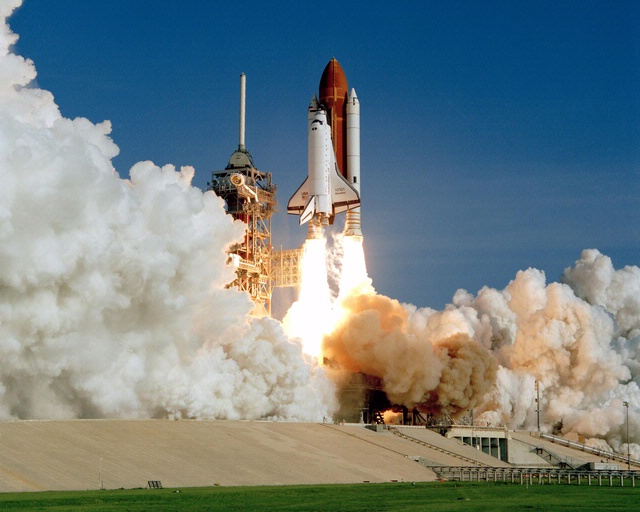
\includegraphics[scale=0.35]{gambar/roketluarangkasa.jpg}

%  % Ubah dengan keterangan gambar yang diinginkan
%  \caption{Peluncuran roket luar angkasa \emph{Discovery} \citep{roketluarangkasa}.}
%  \label{fig:roketluarangkasa}
%\end{figure}

%Roket luar angkasa merupakan \lipsum[1]

%\emph{Discovery}, Gambar \ref{fig:roketluarangkasa}, merupakan \lipsum[2]

% Per Teori Penunjang dibuat section baru

%\section{Gravitasi}
%\label{sec:gravitasi}

\subsection{YOLO}
\label{subsec:YOLO}
YOLO (You Only Look Once) merupakan sistem deteksi objek secara waktu nyata. YOLO merupakan single CNN (Convulotional Neural Network) yang secara bersamaan memprediksi lebih dari satu bounding boxes dan kelas pada satu gambar dalam satu kali pindai. Framework ini dikembangkan oleh Redmon J., Divvala S., Girshick R., Farhadi A. arsitektur jaringannya terinspirasi dari model GoogLeNet untuk klasifikasi gambar. jaringan YOLO memiliki 24 convolutional layer diikuti dengan dua layer yang terhubung.
Saat ini, ada tiga versi YOLO yaitu YOLOv1, YOLOv2, dan YOLOv3. YOLOv2 merupakan versi yang telah dikembangkan dari YOLOv1 yang mana tetap memiliki kecepatan yang sama namun dengan penambahan batch normalization, anchor boxes dan high-resolution classifier. pada YOLOv3, fitur ektraksi yang lebih baik diperkenalkan dilanjutkan dengan perkenalan 53 convolutional layer terlatih pada ImageNet. Tingkat ketelitian YOLOv3 lebih baik dari YOLOv2 namun lebih lambat karena lebih banyak layer.\citep{Redmon_2016_CVPR}

\subsection{Bangun Datar}
\label{subsec:BangunDatar}
Dalam geometri, bentuk 2D didefinisikan sebagai bangun datar yang hanya memiliki dua dimensi yaitu panjang dan lebar. Mereka tidak memiliki ketebalan apapun dan hanya dapat diukur dengan dua dimensi. Lingkaran, persegi, persegi panjang, dan segitiga adalah beberapa contoh benda dua dimensi dan bentuk-bentuk ini dapat digambar di atas kertas. Semua bentuk 2D memiliki sisi, simpul (sudut), dan sudut internal, kecuali lingkaran, yang merupakan sosok melengkung. Bentuk 2D dengan setidaknya tiga sisi lurus disebut poligon dan itu termasuk segitiga, bujur sangkar, dan segi empat.\citep{BRIBIESCA1992483}

%\subsection{Hukum Newton}
%\label{subsec:hukumnewton2}
% Contoh pembuatan persamaan
%\begin{equation}
%  \label{eq:hukumpertamanewton}
%  \sum \mathbf{F} = 0\; \Leftrightarrow\; \frac{\mathrm{d} \mathbf{v} }{\mathrm{d}t} = 0.
%\end{equation}

%\subsection{Anti Gravitasi}
%\label{subsec:antigravitasi}
\subsection{CNN}
\label{subsec:CNN}
Metode CNN (Convolutional Neural Network) merupakan pengembangan dari Metode
Multilayer Perceptron (MLP) yang didesain untuk mengolah data dua dimensi. Cara kerja CNN
memiliki kesamaan pada MLP, namun dalam CNN setiap neuron dipresentasikan dalam
bentuk tiga dimensi, tidak seperti MLP yang setiap neuron hanya berukuran satu dimensi.
Terdapat beberapa arsitektur CNN yang umum digunakan. Arsitektur tersebut yaitu
LeNet, AlexNet, ZF Net, GoogLeNet, VGGNet dan ResNet. CNN terdiri dari tiga jenis layer,
yaitu convolutional layer (Conv), pooling layer (Max pooling) dan fully-connected layer (Full
Connection). Tumpukan lapisan tersebut membentuk arsitektur dari CNN.\citep{DBLP:journals/corr/OSheaN15}

  \cleardoublepage

  % Bab 3 desain dan implementasi
  \chapter{METODOLOGI}
\label{chap:metodologi}

% Ubah bagian-bagian berikut dengan isi dari desain dan implementasi
% Ubah konten-konten berikut sesuai dengan isi dari metodologi

\section{Data dan Peralatan/ Data dan Alat Bantu/ Material }

% Berikut merupakan data dan perlatan yang mendukung pengerjaan Tugas Akhir ini.
\begin{itemize}
	\item [$\bullet$]Dataset berupa gambar bangun datar segitiga, persegi, persegi panjang, lingkaran, dan trapesium berjumlah 50 gambar untuk tiap bangun datar
	
	% \begin{figure} [H] \centering
		%   % Nama dari file gambar yang diinputkan
		%   \includegraphics[scale=0.2]{gambar/UTKFace.png}
		%   % Keterangan gambar yang diinputkan
		%   \caption{Dataset UTKFace}
		%   % Label referensi dari gambar yang diinputkan
		%   \label{fig:UTKFace}
		% \end{figure}
	
	\item [$\bullet$]Dataset berupa gambar tulisan parameter bangun datar 
	\begin{itemize}
		\item [$\bullet$]Untuk bangun datar segitiga parameternya adalah huruf a(alas) dan t(tinggi) berjumlah 50 gambar untuk tiap huruf
		\item [$\bullet$]Untuk bangun datar persegi parameternya adalah huruf s(sisi) berjumlah 50 gambar untuk tiap huruf
		\item [$\bullet$]Untuk bangun datar persegi panjang parameternya adalah huruf P(panjang) dan L(lebar) berjumlah 50 gambar untuk tiap huruf
		\item [$\bullet$]Untuk bangun datar lingkaran parameternya adalah huruf R(jari-jari) berjumlah 50 gambar untuk tiap huruf
		\item [$\bullet$]Untuk bangun datar trapesium parameternya adalah huruf a(sisi atas), b(sisi bawah), dan T(tinggi) berjumlah 50 gambar untuk tiap huruf
		\item [$\bullet$]Angka untuk parameter (1,2,3,4,5,6,7,8,9,0) berjumlah 50 gambar untuk tiap angka
	\end{itemize}
	
	\item [$\bullet$]Roboflow sebagai alat untuk melabeli atau memberikan anotasi pada gambar yang akan digunakan untuk melatih model YOLO.
	\item [$\bullet$]Kamera \\
	
\end{itemize}


\section{Metodologi Penelitian}
% Metodologi yang digunakan dalam pengerjaan Tugas Akhir ini adalah sebagai berikut.
% Contoh input gambar dengan format *.jpg
\begin{figure}[ht]
	% Nama dari file gambar yang diinputkan
	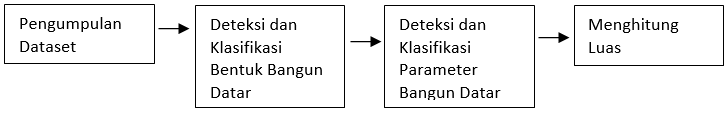
\includegraphics[scale=0.7]{gambar/Metodologi.png}
	% Keterangan gambar yang diinputkan
	\caption{Diagram blok metodologi}
	% Label referensi dari gambar yang diinputkan
	\label{fig:Metodologi}
\end{figure}

\begin{enumerate}
	\item \textbf{Pengumpulan Data} \\
	Pengumpulan dataset dilakukan dengan menggambar bangun datar dan parameter bangun datar pada papan tulis lalu disimpan dalam bentuk foto. lalu melakukan pelabelan pada objek yang ingin dideteksi
	\item \textbf{Deteksi dan Klasifikasi Bentuk Bangun Datar} \\
	Citra diproses dari kamera lalu program akan mendeteksi dan mengklasifikasi bentuk bangun datar.
	\item \textbf{Deteksi dan Klasifikasi Parameter Bangun Datar} \\
	Citra diproses dari kamera lalu program akan mendeteksi dan mengklasifikasi parameter bangun datar..
	\item \textbf{Menghitung Luas} \\
	Dari hasil deteksi dan klasifikasi, program akan melakukan perhitungan luas sebuah bangun datar.
\end{enumerate}





%Penelitian ini dilaksanakan sesuai \lipsum[1][1-5]


%\section{Peralatan}
%\label{sec:peralatan}

%Alat yang digunakan yaitu: \lipsum[1]

%\subsection{Perangkat}
%\label{subsec:perangkat}

%Perangkat yang digunakan menggunakan spesifikasi \lipsum[1]

%\section{Desain Sistem}
%\label{sec:desainsistem}

%Sistem akan dibuat dengan \lipsum[1-2]

% Per blok diagram dijelaskan dan dibuatkan section masing-masing

% \section{Blok Diagram}
% \label{sec:blokdiagram}

% Contoh pembuatan potongan kode
%\begin{lstlisting}[
%  language=C++,
%  caption={Program halo dunia.},
%  label={lst:halodunia}
%]
%#include <iostream>
%
%int main() {
%    std::cout << "Halo Dunia!";
%    return 0;
%}
%\end{lstlisting}

%\lipsum[2-3]

% Contoh input potongan kode dari file
%\lstinputlisting[
%  language=Python,
%  caption={Program perhitungan bilangan prima.},
%  label={lst:bilanganprima}
%]{program/bilangan-prima.py}

%\lipsum[4]

  \cleardoublepage

  % Bab 4 pengujian dan analisis
  \chapter{HASIL DAN PEMBAHASAN}
\label{chap:hasilpembahasan}

% Ubah bagian-bagian berikut dengan isi dari hasil dan pembahasan

Pada penelitian ini dipaparkan \lipsum[1][1-5]

% Skenario pengujian berupa hasil penelitian dan perancangan yang telah dibuat pada bab 3

\section{Skenario Pengujian}
\label{sec:skenariopengujian}

Pengujian dilakukan dengan \lipsum[1-2]

\section{Evaluasi Pengujian}
\label{sec:analisispengujian}

Dari pengujian yang \lipsum[1]

% Contoh pembuatan tabel
\begin{longtable}{|c|c|c|}
  \caption{Hasil Pengukuran Energi dan Kecepatan}
  \label{tb:EnergiKecepatan}\\
  \hline
  \rowcolor[HTML]{C0C0C0}
  \textbf{Energi} & \textbf{Jarak Tempuh} & \textbf{Kecepatan} \\
  \hline
  10 J & 1000 M & 200 M/s \\
  20 J & 2000 M & 400 M/s \\
  30 J & 4000 M & 800 M/s \\
  40 J & 8000 M & 1600 M/s \\
  \hline
\end{longtable}

\lipsum[2-4]

  \cleardoublepage

  % Bab 5 penutup
  \chapter{PENUTUP}
\label{chap:penutup}

% Ubah bagian-bagian berikut dengan isi dari penutup

\section{Kesimpulan}
\label{sec:kesimpulan}

Berdasarkan hasil pengujian yang \lipsum[1][1-3] sebagai berikut:

\begin{enumerate}[nolistsep]

  \item Pembuatan \lipsum[2][1-3]

  \item \lipsum[2][4-6]

  \item \lipsum[2][7-10]

\end{enumerate}

\section{Saran}
\label{chap:saran}

Untuk pengembangan lebih lanjut pada \lipsum[1][1-3] antara lain:

\begin{enumerate}[nolistsep]

  \item Memperbaiki \lipsum[2][1-3]

  \item \lipsum[2][4-6]

  \item \lipsum[2][7-10]

\end{enumerate}

  \cleardoublepage

  % Daftar pustaka
  \renewcommand\bibname{DAFTAR PUSTAKA}
  \addcontentsline{toc}{chapter}{\bibname}
  \bibliographystyle{unsrtnat}
  \bibliography{pustaka/pustaka.bib}
  \cleardoublepage

  % Biografi penulis
  \begin{center}
  \Large
  \textbf{BIOGRAFI PENULIS}
\end{center}

\addcontentsline{toc}{chapter}{BIOGRAFI PENULIS}

\vspace{2ex}

\begin{wrapfigure}{L}{0.3\textwidth}
  \centering
  \vspace{-3ex}
  % Ubah file gambar berikut dengan file foto dari mahasiswa
  
\includegraphics[width=0.3\textwidth]{gambar/elon.jpg}
  \vspace{-4ex}
\end{wrapfigure}

% Ubah kalimat berikut dengan biografi dari mahasiswa
Elon Reeve Musk, lahir pada \lipsum[1]

\lipsum[2]

  \cleardoublepage

\end{document}
